%!TEX root = ../BoYu-Dissertation.tex
\graphicspath{{Figures/}}

\chapter{Awareness Promotion} % (fold)
\label{cha:awareness_promotion}
The conceptual model of awareness presented in the previous chapter clearly shows the increased complexity of the awareness phenomena in complex, distributed collaborative activities:

\begin{enumerate}
   \item First, due to the highly distributed nature of the collaborative activities, team members play specialized roles and are engaged in different actions. As a result, each actor has distinct awareness requirement, related to the goals and actions that they are working towards.
   \item Second, in order to achieve the compatible awareness at the team level, each actor needs to be aware of more things than their individual awareness, and spare extra effort to interact with each other.
   \item Last, because of the continuous development of the collaborative activities, the actors' awareness requirements are quite fleeting.
\end{enumerate}

As a result, awareness can no longer be achieved effortlessly by the actors themselves, and computer support can play an important role to augment and complement human capability. This chapter provides the overview of our computational approach to supporting awareness in complex, distributed collaborative activities. The general design principle of our approach is to emphasize the active role of computer system to not merely support, but rather promote awareness in collaborative activities.

In this chapter, we first identify the major challenges for human actors to achieve and develop awareness in distributed, complex collaborative activities, which highlight the design aspects in which computer systems can provide support. Then we discuss how these design aspects have been addressed (or partially addressed) in existing awareness supporting systems. Last, we present our computational awareness promotion framework that has the potential to better address these challenges.

\section{Designing for awareness support} % (fold)
\label{sec:designing_for_awareness_support}
As described in Section \ref{sec:awareness_processes}, in order to achieve awareness, human actors have to engage in a variety of awareness processes at both the individual and team levels. In this section, we identify the major cognitive and interactive challenges for human actors in these awareness processes, and analyze how the computer system can provide support to address these challenges correspondingly.

\subsection{Support for individual awareness} % (fold)
\label{sub:support_for_individual_awareness}
\paragraph*{Perception} % (fold)
\label{par:perception}
The achievement of individual awareness starts with the ability of individuals to perceive key awareness elements in the environment. As the complexity of the collaborative activities scales up, there are potentially a very large number of awareness elements that are available at any given time. However, due to the partiality of individual awareness, each actor is only interested in a small set of them that are relevant to his/her own task. As a result, human actors have to focus on filtering out a large number of irrelevant information, which may consume too much of the actor's attention. 

The computer can support the human actors in this process by reducing the number of awareness elements presented to the actors. If the system can predict the awareness needs of the actors, the effort of filtering out irrelevant information can be transferred to the computer systems, so that human actors can focus on processing only the relevant set of information to avoid information overload.
% paragraph perception (end)

\paragraph*{Comprehension} % (fold)
\label{par:comprehension}
Comprehension is to understand the meaning of perceived awareness information within the context of an actor's current actions \cite{oulasvirta2007a}. In the comprehension process, new awareness information must be combined with existing knowledge about the current collaborative activity, which provides the inferential framework \cite{carroll2003a} for the actor to evaluate which part of the collaborative activity will be impacted by the perceived awareness information. 

Without computer support, human actors have to maintain existing knowledge about the collaborative activities in their minds. However, in complex, collaborative activities where the magnitude of the collaborative work can grow significantly as hundreds or thousands of actors engaged in myriads of interdependent actions, it becomes a challenging task for human actors to maintain such an inferential framework in the mind. Alternatively, there are two ways that the comprehension can be supported by computer systems: 

\begin{enumerate}
   \item First, the computer system can support human comprehension by providing external representations of the existing knowledge. Instead of merely relying on the internal representations of human users, the external representation can serve as the information store, so that the internal representation at a given time can be quite sparse, perhaps containing only detailed information about their current focus \cite{Hegarty2011}, or pointers to locations of other important information in the external representation \cite{M.1996}. In this way, the limited working memory resource of human users is freed up for other aspects of cognition \cite{M.1996}.
   \item Second, the computer system can directly aid the linking between new awareness information and existing knowledge by presenting the awareness information along with the contextual information that is potentially relevant to understand its meaning \cite{Tomaszewski2010}. Supporting comprehension by linking has its basis on the design principle of offloading cognitive processes onto perceptual processes \cite{M.1996}. By explicitly linking the awareness information to contextual information for interpretation, some complex cognitive processes, such as searching for and activating the relevant portion of existing knowledge, can be replaced by simple pattern recognition processes \cite{Hegarty2011}. 
\end{enumerate}
% paragraph comprehension (end)

\paragraph*{Projection} % (fold)
\label{par:projection}
Projection is the process that the individual predicts the future states of other actions based on the comprehension of awareness information. As argued by Endsley \cite{Endsley1995}, this is the most difficult and taxing part to achieve individual awareness because it requires a fairly well developed mental model of the actions and relationships among them, along with the capabilities to perform reasoning. The analytical reasoning is central to the projection process, through which the actors explore possible alternative future scenarios and identify the one most likely to come \cite{Thomas2006}. Similar to the comprehension process, when the complexity of collaborative activities scales up, it becomes a challenging cognitive task for human actors due to the large volume of knowledge that needs to be stored and consumed during the reasoning process. The computer support for projection, as a result, can be supported from two aspects:

\begin{enumerate}
   \item The projection process can also be supported by providing external representations of existing knowledge and the analytic tools to allow the actors to synthesize information and derive insight from it.
   \item On the other hand, the system can perform the reasoning tasks on behalf of human actors, and simply present the reasoning results to them. In this way, the high level reasoning tasks are transformed into low level perceptual tasks for the actors.
\end{enumerate}
% paragraph projection (end)
% subsection support_for_individual_awareness (end)
\subsection{Support for collaborative awareness} % (fold)
\label{sub:support_for_collaborative_awareness}
As we described in Section \ref{sub:development_of_collaborative_awareness}, the development of collaborative awareness is mediated by the transactions between multiple actors through which actors' individual awareness processes are connected as developmental trajectories. As a result, besides the individual awareness processes, the actors have to perform the team processes to conduct awareness transactions.

The challenges for actors to perform the team processes for awareness development can be analyzed from two aspects: the overhead of maintaining additional transactive knowledge and the extra effort to perform them. 

\paragraph*{Transactive knowledge} % (fold)
\label{par:transactive_knowledge}
In order to conduct awareness transactions, the actors need to attain more knowledge than what is needed for their individual work. In general, we can identify two types of knowledge that are necessary for the actors to conduct awareness transactions.
\begin{enumerate}
   \item First is related to the concept of `transactive memory' that describes how the individual memories of team members are supplemented by the additional knowledge about other actors \cite{wegner1987transactive}. Within the context of collaborative awareness, that means, in order to conduct awareness transactions, the actors need to maintain knowledge about how each other's work is related. To monitor each other's work, the actors need to know who else's work can potentially impact their own work. To externalize or communicate their individual awareness to others, the actors need to know whose work may be impacted.  
   \item The other is knowledge about the historical development of awareness. The awareness information perceived by an actor may not be directly generated from the environment, rather it can be the result of multiple awareness transactions across several actors. In order to understand the meaning of the perceived awareness information, the actor has to trace back to understand where it comes from, who else has been impacted or contributes to its development, etc.
\end{enumerate}

As the complexity of collaborative activities scales up, maintaining these two types of knowledge increases the actors' cognitive overhead significantly. With the increased number of actors and possible dependencies among their actions, the knowledge about other actors whose actions are related to an actor grows rapidly. In addition, there are more actors participated in each developmental trajectory, so that it becomes difficult for the actors to keep track of the historical development of awareness.

Correspondingly, the computer system can support the actors by maintaining these two types of transactive knowledge for them. Whenever the actors need the knowledge, they can turn to the computer system to retrieve it. Moreover, the computer system can make use of the knowledge on behalf of human actors and perform reasoning to facilitate the awareness transactions. If the computer system knows whose actions to monitor, the system can monitor them for the actors. If the computer knows who needs to be notified by a piece of awareness information, it can deliver it to the relevant actors without human intervention.
% paragraph transactive_knowledge (end)

\paragraph*{Team processes} % (fold)
\label{par:team_processes}
Besides the additional knowledge that is needed, awareness transactions are often achieved by some sort of team processes, such as direct communication or externalization in which the actors make aspects of their individual awareness visible to others. These team processes pose an additional effort to the actors who initiate the awareness transactions. Moreover, the actors who perform these team processes, i.e. the \emph{initiators} of team transactions, are often not the actors who will directly benefit from them. The disparity between cost and benefit \cite{Grudin1994} becomes an important challenge for the awareness development, as it may discourage the actors to conduct the awareness transactions. As a result, in order to support the development of collaborative awareness, the computer system needs to provide effective tools for the actors to perform the team processes, so that the extra effort can be minimized.
% paragraph team_processes (end)
% subsection support_for_collaborative_awareness (end)

Table \ref{tab:design_aspects} summarizes the major challenges for human actors and the design aspects for computer systems to support the awareness processes.

%\needspace{8\baselineskip}
% \clearpage

\begin{table}[htbp]
\centering
\footnotesize
\begin{tabular}{>{\raggedright}p{1.2in}>{\raggedright}p{2.2in}>{\raggedright}p{2.2in}}
\toprule 
\textbf{Awareness Process} & \textbf{Challenges for human actors} & \textbf{Design aspects for computer support}\tabularnewline
\midrule 
\multirow{3}{1.2in}{Development of individual awareness} & \emph{Perception}: they have to filter out a large number of irrelevant
information, consuming their attention resources & \emph{1.} \emph{Filtering}: the computer predicts the awareness needs
and filters out irrelevant information for human actors.\tabularnewline
\cmidrule{2-3} 
 & \emph{Comprehension}: they have to maintain a large volume of knowledge
about the collaborative activities in their minds & \emph{1. Representation}: the computer provides external representations
of the existing knowledge to free up human working memory resources.

\emph{2. Linking}: the computer presents the awareness information
along with the contextual information that is potentially relevant
to understand its meaning.\tabularnewline
\cmidrule{2-3} 
 & \emph{Projection}: they have to maintain the large volume of existing
and derived knowledge during the reasoning process  & \emph{1. Representation}: the computer provides external representations
and analytic tools to allow the human actors to synthesize information
and derive insight.

\emph{2. Reasoning}: the computer performs the reasoning tasks and
presents the reasoning results to human actors.\tabularnewline
\midrule 
\multirow{3}{1.2in}{Development of collaborative awareness} & \emph{Transactive knowledge}: they need to maintain transactive knowledge
that increases their cognitive overhead significantly & \emph{1. Representation}: the computer provides external representations
of the transactive knowledge.

\emph{2. Reasoning}: the computer makes use of the knowledge on behalf
of human actors and performs reasoning to facilitate awareness transactions.\tabularnewline
\cmidrule{2-3} 
 & \emph{Team processes}: they need to spare additional effort to conduct
team processes, but are often not the actors who will directly benefit
from them. & \emph{1. Tools}: the computer needs to provide the tools that simplify
the effort to perform team processes.\tabularnewline
\bottomrule
\end{tabular}  
\caption{Design aspects for awareness support}
\label{tab:design_aspects}
\end{table}


% section designing_for_awareness_support (end)

\section{Existing studies} % (fold)
\label{sec:the_state_of_art}
By outlining the design aspects for awareness support in Section \ref{sec:designing_for_awareness_support}, we can use them to review existing awareness supporting systems by looking into how these design aspects have (or have not) been supported. Before that, we need to make a distinction between two types of computational models for organizing and processing awareness information: \emph{space-based} and \emph{event-based} models, because it is the underlying computational model that determines how the awareness processes are supported in an awareness system \cite{Gross2004}.

\subsection{Computational models of awareness support} % (fold)
\label{sub:awareness_models}
Most awareness systems rely on certain computational models to organize and process awareness information. A computational model usually provides a representation of the collaborative work, and specifies how awareness information is generated on top of it. In general, we can distinguish two types of awareness models commonly used in existing awareness systems: \emph{space-based} and \emph{event-based} models. 

\subsubsection{Space-based models} % (fold)
\label{ssub:space_based_model}
Many researchers have previously described systems to support awareness based on the spatial metaphor \cite{Benford1993,Rodden1996,Sandor1997,simone2002a}. These space-based models explicitly represent the various shared objects, such as actors, information, resources, or other computer artifacts, situated and manipulable in some space. Awareness is then achieved by the interaction between actors, as they present themselves and attend to each other in the space \cite{Rodden1996}. Awareness information thus is implicitly embedded as perceivable properties of objects in the space.  

The use of space-based model relies on presenting a `shared space' among collaborators at any given time to provide awareness information, both implicitly and explicitly \cite{dourish1992awareness}. By maintaining the state of the shared work setting, people can either keep an eye on what the rest of the group is doing while doing their individual work, or actively monitor the actions of others, to perceive awareness information \cite{simone2002a}. 
In existing awareness systems, the `shared space' can take different forms \cite{antunes2010a}. 
\begin{enumerate}
   \item `Shared physical space'. In the early work of supporting awareness, a significant effort was devoted to exploring the potential of media space technologies, i.e. an array of continually audio-video links between distributed actors, to provide a `shared physical space' between actors in different locations \cite{Dourish1992}. As with the awareness study, the media space investigations were concerned with informal or social aspect of awareness, and in most cases task-oriented awareness was not mentioned explicitly \cite{schmidt2002a}.
   \item `Shared virtual space'. Rodden \cite{Rodden1996} developed the notion of `virtual space' as a collection of computer-supported interactive spaces. Many collaborative systems offer various types of virtual spaces to support awareness, including abstract media space \cite{Pedersen1997}, virtual meeting rooms \cite{Berlage1999}, and collaborative virtual environment \cite{Benford2001}. Unlike traditional media spaces that aim to establish the `shared physical space', this line of work focuses on the use of abstract representations as awareness indicators. Besides providing a kind of `shielding' for privacy of the people in the shared space \cite{Pedersen1997}, a more interesting feature of using abstract representations is the capability to organize awareness information around task-oriented structures, such as office tables, meeting rooms \cite{Berlage1999}, so that more task-oriented aspects of awareness can be supported.
   \item `Shared workspace'. `Shared workspace' is a specialization of the notion of `shared space' that emphasizes the task-oriented awareness. According to Gutwin and Greenberg \cite{Gutwin2002}, a `shared workspace' is a bounded space where people can see and manipulate artifacts related to their activities. A group editor is a good example of this type of `shared workspace', as it serves to organize activities like writing and revising, while maintaining a coherent view of the whole \cite{dourish1992awareness}. The awareness information in `shared workspace' is presented by attaching it to the manipulable objects through which the task is carried out, and is achieved by user's interaction with the artifacts \cite{Gutwin2002}.
\end{enumerate}
% subsubsection space_based_model (end)

\subsubsection{Event-based models} % (fold)
\label{ssub:event_based_model}
\emph{Event-based} models, on the other hand, provide people with awareness of what is going on around them as expressed by discrete events \cite{rittenbruch2009a}. Each event highlights a piece of awareness information related to certain state change in a collaborative setting for a limited amount of time. Events can be generated by sensors that are associated with actors, shared material, or any other objects that constitute or influence a cooperative environment \cite{prinz1999a}. The list of events that are supported in each awareness system can be totally different, depending on the application domain. As argued by Fuchs et al \cite{Fuchs1995}, we can basically imagine any kind of events, as long as it has a certain relevance when it comes to coordinating the work in a given setting. 

Unlike space-based models where the awareness information is implicitly embedded as properties of objects in the underlying representation of shared spaces, awareness information is explicitly represented as first-class objects in event-based models. Each event contains identifiers of the originator, the time, the state change in the collaborative setting, and the context in which the state change took place \cite{fuchs1999a}. Modeling awareness information as first-class objects decouples it from the objects or artifacts in the collaborative activities, which provides several distinguishing features from the space-based models:

\begin{enumerate}
   \item It allows the awareness information referring to any aspects of collaborative activities, not only the external aspects, but also the internal aspects reflecting the intentions and beliefs of actors.
   \item The awareness information is not limited within the user's current viewpoint. The user may attend to their own individual work in the filed, but still be able to receive events about other users that are outside his/her current viewpoint. 
   \item The awareness information is pushed to the actors when the event happens, so that they do not need to spare their attentional resource to monitor each other's work.
\end{enumerate}

Because of the decoupling of awareness information from the representation of collaborative work, many existing event-based systems actually do not need to provide an explicit shared representation of the collaborative work \cite{prinz1999a,Fitzpatrick2002}.  Even in some systems where the collaborative work is represented (for example, the GroupDesk \cite{Fuchs1995} and the POLIAwaC systems \cite{sohlenkamp2000po} use semantic networks comprised of actors, artifacts, events, and their relations; the BSBW system \cite{Bentley1995} and Atmosphere model \cite{Rittenbruch2002} use hierarchical structures of workspaces), they are mainly used by the designers to specify events and manage event distributions, and are invisible to the actors.
% subsubsection event_based_model (end)

Table \ref{tab:awareness_models} shows a summary of the major distinguishing features of the \emph{space-based} and \emph{event-based} models. In the following of this section, we will discuss details on how the design aspects in various cognitive and social processes as shown in Section \ref{sec:designing_for_awareness_support} have (or have not) been supported each of these models.

\begin{table}[htbp]
\centering
\footnotesize
\begin{tabular}{>{\raggedright}p{1.1in}>{\raggedright}p{2.2in}>{\raggedright}p{2.2in}}
\toprule 
 & \textbf{Space-based models} & \textbf{Event-based models}\tabularnewline
\midrule 
Representation of the collaborative work & explicitly represented as a `shared space' inhabited by objects representing
actors, information, resources, or other computer artifacts  & implementation-dependent internal representations\tabularnewline
\midrule 
\multirow{4}{1.1in}{Awareness information} & embedded as perceivable properties of objects in the space & explicitly represented as discrete events\tabularnewline
\cmidrule{2-3} 
 & limited to external aspects of shared objects  & can refer to both external and internal aspects\tabularnewline
\cmidrule{2-3} 
 & presented in the context of its origin & can be outside the user's current viewport\tabularnewline
\cmidrule{2-3} 
 & users need to pull the awareness information from the field of work & awareness information is pushed to the users\tabularnewline
\midrule 
Example Implementations & 1. physical spaces (e.g. Portholes \cite{Dourish1992})

2. virtual spaces (e.g. AROMA \cite{Pedersen1997},
DIVA \cite{Berlage1999}, MASSIVE-2 \cite{Benford2001})

3. workspaces (e.g. ShrEdit \cite{dourish1992awareness},
GroupKit \cite{Roseman1996}) & GroupDesk \cite{Fuchs1995}, POLIAwaC \cite{sohlenkamp2000po},
NESSIE \cite{prinz1999a}, Elvin \cite{Fitzpatrick2002}\tabularnewline
\bottomrule
\end{tabular}  
\caption{The main distinguishing features of space-based and event-based models}
\label{tab:awareness_models}
\end{table}

One thing to note is that, in many existing awareness systems, the space-based and event-based models are not exclusive, rather they are combined together to provide an integrated awareness supporting environment. Many shared workspace systems, such as the GroupDesk \cite{Fuchs1995}, the POLIAwaC \cite{sohlenkamp2000po}, and the ENI \cite{Gross2004} systems, present a shared workspace among the collaborators, and at the same time support event notifications. Atmosphere model \cite{Rittenbruch2002} uses hierarchical structures of workspaces, i.e. spheres, to represent the shared collaborative work, and they are also used to specify events and manage event distributions.
% subsection awareness_models (end)

\subsection{Awareness support in existing systems} % (fold)
\label{sub:awareness_support_in_existing_systems}

\subsubsection{Support for perception} % (fold)
\label{ssub:support_for_perception}
The support for perception regards filtering awareness information for human actors, which has been described in both \emph{space-based} and \emph{event-based} systems.

\paragraph*{Space-based systems} % (fold)
\label{par:space_based_systems}
Systems adopting the space-based awareness model usually depend on the various relationships between objects inhabiting in the shared space to decide on the relevance of awareness information.

Benford et al.'s spatial model \cite{Benford1993} provides a formal approach to managing awareness levels between objects inhabiting in a common spatial frame. Awareness between objects is manipulated via \emph{focus} and \emph{nimbus}, two subspaces within which an object chooses to direct either its presence or its attention. Then the awareness information is selected based on the overlapping between the receiver's \emph{focus} and the performer's \emph{nimbus} in certain medium \cite{Benford1993}. Anything about the performer happens in the overlapping area will be perceivable to the receiver. 

The original spatial model has been extended in several ways to support different awareness systems. Sandor et al. \cite{Sandor1997} redefined the concepts of \emph{focus} and \emph{nimbus} upon a semantic network that forms a representation of the working context, and use them to build a generic model `Aether' for supporting awareness in collaborative systems. Rodden \cite{Rodden1996} adopted an object-oriented approach to generalize the spatial model to provide notions of presence, sharing and awareness applicable to applications lacking a spatial metaphor. Simon and Bandini \cite{simone2002a} based on the spatial mode to propose the reaction-diffusion model that can support more user adaptation and dynamic features. Instead of using \emph{focus} and \emph{nimbus}, the awareness information is distributed using field and sensitivity function that allow for a more flexible and compact way of representing various types of nimbi and foci. 

Although various space-based models differ from each other in the specific calculation of awareness levels, the most important point emphasized in all of this work is the insistence that the selection of awareness information is a joint-product between the performer and the receiver, i.e. how the receiver directs the attention to the performer (\emph{focus}) and how the performer projects the presence or activity to the receiver (\emph{nimbus}).
% paragraph space_based_systems (end)

\paragraph*{Event-based systems} % (fold)
\label{par:event_based_systems}
Filtering awareness information in event-based systems focuses on managing events subscriptions that are used by human actors to describe their awareness interests. Many mechanisms that enable the event subscriptions have been discussed in the literature, and they vary from each other depending on how the filters are defined. 

\begin{enumerate}
   \item \emph{Type-based filtering}. In the GroupDesk system \cite{Fuchs1995}, Fuchs et al. define several filters that allow the limit of the flow of events. Definition of these filters is based on individual event types, which consist of a mapping from a set of event types to a list of interested users. The drawback of type-based filtering is that it requires the user to explicit his/her interest on each event type in a predetermined way, which is a tedious task that the users are not always willing to perform \cite{Grudin1994}. Furthermore, the type-based subscriptions tend to be too rigid or unable to adapt to the team development \cite{Alarcon2002}.
   \item \emph{Content-based filtering}. Alternatively, Elvin \cite{Fitzpatrick2002} adopts the content-based filtering of events. It describes events using a set of named attributes of simple data types and consumers subscribe to sets of events using boolean subscription expressions. When a notification is received at the Elvin server from a producer, it is compared to the consumers' registered subscription expressions and forwarded to those whose expressions it satisfies. A key benefit of content-based filtering is the increased expressiveness to describe interests. Users can subscribe to event patterns, which can describe a set of events based on their attributes, rather than pre-defined event types.
   \item \emph{Context-based filtering}. ENI \cite{Gross2004} extends the content-based filtering approach and integrates the notion of `contexts' into the model. Context information includes locations, artifacts and applications and other information, which is linked to a specific context. ENI adds this information to existing event information in an awareness system. The model is based on two concepts of context. First, the model tries to determine the context of origin for each event. The authors suggest a context mapping mechanism that maps events gathered from sensor information against rules saved in a context database. Second, the model identifies the work context of the user who is receiving the notification. The work context is derived from the selection of shared workspaces. Based on the two types of context, then the filtering is performed on context matching, i.e. the user defines what types of event context he/she wants to receive in a specific work context. The context-based model tries to improve the event filtering by gathering additional information and allowing users to receive awareness information in a more context-specific manner. However, the context mapping mechanisms underlying this concept is highly complex, and it lacks a formal model to specify the two types of context.
\end{enumerate}
% paragraph event_based_systems (end)

\paragraph*{Comparison} % (fold)
\label{par:comparison}
The space-based systems rely on the users to monitor the shared spaces and perceive the relevant awareness information. As the whole field of work as a shared space is explicitly visible to each user, they can pick up the awareness information relevant to them even when their own interests have been changed. This provides more flexibility to handle increased level of dynamics. However, space-based systems become much more problematic when the level of complexity in collaborative activities increases as well. When the numbers of objects, actors and their actions are significantly increased, representing them in a shared space and relying on the users to monitor and filter awareness information from it becomes a challenging task.

Event-based model provides a more lightweight way to present awareness information, as only the aspects of awareness information that is of relevance are presented. Furthermore, the event-based presentation is pushed to the users by making the events more perceivable to the users. In this way, the users do not need to switch their attention to other's actions until the event notification happens. As a result, event-based models can handle more complex situations than space-based models. However, the effectiveness of event-based models largely depends on the quality of event subscriptions, which often requires that considerable domain knowledge be explicitly embedded. As argued by Fuchs et al. \cite{fuchs1999a}, event-based systems seem to work satisfactorily for situations where workflow can be clearly defined in advance or if the application is known from the beginning. When the level of dynamics increases in collaborative activities, such condition can no loner hold. The user's awareness needs are often in the flux of changes, as their activities evolve. Hence, event-based systems become less effective to handle high level of dynamics.
% paragraph comparison (end)
% subsubsection support_for_perception (end)

\subsubsection{Support for comprehension} % (fold)
\label{ssub:support_for_comprehension}
The computer support in the comprehension process comes from two aspects: providing external representations of existing knowledge to free up human working memory resources, and linking the awareness information along with the contextual information that is potentially relevant to understand its meaning.

\paragraph*{Space-based systems} % (fold)
\label{par:space_based_systems}
Most existing space-based systems provide visual-spatial displays \cite{Hegarty2011} of the shared spaces, which has a number of advantages to support comprehension. First, they organize information by indexing it spatially. In these displays, space in the display represents space in the field of work, so that if the representation of two items is close in the display, it is likely that those items are also close in the represented field of work. Therefore, information that needs to be related in interpreting and making inferences is likely to be represented by visual features that are close in the display \cite{Hegarty2011}. Second, they provide overview of the whole field of work, and therefore can be perceived as a whole and provide necessary background for comprehending awareness information \cite{Berlage1999}. Furthermore, as the awareness information can be directly presented in the place of its origin, the user can offload the cognitive effort to locate the related objects onto perceptual processes \cite{M.1996}.

However, space-based systems also have limitations in supporting comprehension. First, we need to distinguish the difference between the context of \emph{origin} of the awareness information and the context of \emph{work} of the user \cite{Gross2004}. Most space-based systems present the awareness information in place of the object where the information occurs on, i.e. within the context of its origin. However, what is more important in the comprehension process is for the user to understand the effects of the awareness information on his/her own work, i.e. within the context of the user's work. Second, the visual-spatial display of the whole field of work can become a difficult or even impractical task when the number of actors, artifacts, and activities increases significantly. 
% paragraph space_based_systems (end)

\paragraph*{Event-based systems} % (fold)
\label{par:event_based_sytems}
Event-based systems often do not provide explicit representation of the field of work. As a result, in order for the user to comprehend an event, he/she has to build and maintain a mental model of the inferential framework derived from the field of work, which increases the cognitive load for the user. To alleviate this problem, some event-based systems attempt to collocate event notifications within the context of work. For example, NESSIE provides the awareness information by the presentation of pictorial activity indicators for the members of a group as part of the shared workspace user interface \cite{prinz1999a}. In the virtual school project, Carroll et al. suggest that external events should be collocated with process and planning representations \cite{carroll2003a}. However, studies on supporting comprehension of events are still very limited. Questions such as what types of events should be collocated with what types of contextual representations are largely undetermined.
% paragraph event_based_systems (end)

\paragraph*{Comparison} % (fold)
\label{par:comparison}
Support for comprehension can be achieved relatively effortlessly in space-based systems because of two features: the existence of an explicit representation of the shared space, and the possibility of presenting awareness information directly in the shared space. Comparing with space-based systems, the comprehension of events provides a more challenging task for the users, as the awareness information is typically presented in separate event-triggered displays peripheral to a person's current task-oriented concern \cite{carroll2003a}. 
% paragraph comparison (end)
% subsubsection support_for_comprehension (end)

\subsubsection{Support for projection} % (fold)
\label{ssub:support_for_projection}
To our knowledge, explicit support for projection is rarely discussed in existing awareness systems. The question about how new awareness information will lead to future changes in human actors' actions is usually considered as a cognitive task that is performed by human users. Since most of the space-based systems provide the external representation of the collaborative work, to some extent it can support projection by providing such an external information store. However, the information represented in these shared spaces is often structured around the objects in the space. Many types of knowledge that is useful to predict future changes, such as the dependency relationships between actions, are not represented.
% subsubsection support_for_projection (end)

\subsubsection{Support for transactive knowledge} % (fold)
\label{ssub:support_for_transactive_knowledge}
Transactive knowledge in space-based systems can be supported by providing lightweight awareness widgets \cite{Gutwin1996}, along with the shared spaces. For example, DIVA uses a virtual office table to display participants in a chat room, as well as visualize their contributions over time\cite{Berlage1999}. The Babble system \cite{Erickson1999} includes a `social proxy' showing team member's level of contribution to a threaded discussion. These awareness widgets represent some aspects of the collaborators, so that the users can check them to figure out who they should interact with, or whether the actors are available for interruption. However, these lightweight awareness widgets only display specific aspects of social awareness, such as the collaborator's arrival, availability, involvement, but cannot adequately support action-oriented awareness aspects \cite{carroll2003a}, such as the predicated status of their actions, the reasons behind their actions, or dependency relations between actions.

In event-based systems, transactive knowledge is usually represented as events that are related to the actors and their actions. For example, in AERE system \cite{fuchs1999a}, the status of other actors' actions is represented as activity events, so that the actors can maintain knowledge about the other participants through the events. However, the actors have to store the information carried in these events in their mind, which is less efficient than the space-based systems. The benefit of event-based system, on the other hand, is the capable to store history information about the awareness development. In many event-based systems, such as GroupDesk \cite{Fuchs1995} and NESSIE \cite{prinz1999a}, an event history is available so that the users can analyze the event history storage to understand how the events are developed. However, most systems store events in the database as individual records, and do not provide links between the events. In order to understand how the events are socially developed through transactions, they have to link them together based on their own interpretations. 
% subsubsection support_for_transactive_knowledge (end)

\subsubsection{Support for team processes} % (fold)
\label{ssub:support_for_team_processes}
As we described in Section \ref{ssub:awareness_transactions}, awareness transactions are supported by three types of team processes: mutual monitoring, direct communication, and externalization.

\paragraph*{Mutual monitoring} % (fold)
\label{par:mutual_monitoring}
In space-based systems, the process of mutual monitoring, i.e. making consequences of individual activities apparent to other participants, can be achieved either through the direct video-audio links between actors \cite{Dourish1992}, or through the artifact mediation \cite{Tee2009}. 

In media space-based systems, monitoring can be supported by the networks of audio and video to provide rich representation of people and their immediate surroundings \cite{Dourish1992}. By seeing others through the media space, it is believed that people can get a sense of others' actions so that they can infer the consequences of their actions. However, Fish et al.'s study in the use of the Cruiser media space \cite{Fish1992} has shown that even though the media space allows the users to perceive each other's actions, it usually does not provide the visibility of the work artifacts involved in these activities. As a result, seeing each other through a media space does not necessarily means the consequences of their actions are visible. 

As a result, a more common approach to mutual monitoring in space-based systems is through the common artifacts in the shared spaces \cite{Berlage1999}. In these systems, users' actions are organized around the common artifacts, which supports the mutual monitoring through feedthrough \cite{dix1997challenges}, i.e., when artifacts are manipulated in some actions, they give off information that informs others the consequences of these actions \cite{Tee2009}. However, artifact-mediated feedthrough is limited to the aspects of users' actions that can be represented as some artifacts, the internal aspects of their actions cannot be supported.

In existing event-based systems, the process of mutual monitoring can be supported by the system's capability to automatically capture events from the environment or the actors. For example, in the GroupDesk \cite{Fuchs1995} system, each time the state of an object changes due to some action of a user, a new event is automatically generated to describe the change. Then the event is sent to the event processing server, and is distributed to the users who subscribe to it. However, the aspects of actions are limited to the external aspects that can be captured by computer systems.
% paragraph mutual_monitoring (end)

\paragraph*{Communication} % (fold)
\label{par:communication}
Computer mediated communication has been an important component in almost every distributed collaborative system, by providing team members a \emph{medium} to communicate with each other remotely \cite{Gutwin2002}. However, it is usually supported separately from the awareness systems as a standalone feature in collaborative applications.
% paragraph communication (end)

\paragraph*{Externalization} % (fold)
\label{par:externalization}
The basic way to support externalization in space-based systems is annotations, which are defined as hypertext nodes that are linked to the objects in the shared spaces \cite{Zheng2006,Weng2004}. Annotations allow the users to add their comments or interpretations on specific objects in the shared space that are visible to other collaborators. In this way, annotations provide a way for the users to externalize their individual awareness and display them to others. However, annotations in space-based systems are often bound to the objects in the shared space, and therefore have limited capability to externalize other aspects of individual awareness, such as the intentions to perform actions, or state changes of actions. 

Rittenbruch et al. introduce and explore the notion of ``intentionally enriched awareness'' \cite{Rittenbruch2007}, which refers to the process of actively engaging users in the awareness process by enabling them to express intentions. ``Intentionally enriched awareness'' emphasizes the role of actors to make some of their internal states (intentions, reasons, etc.) along with their actions visible to others. Their AnyBiff prototypical system is one of the limited existing attempts to support externalization in event-based systems, which allows users to generate, share, and use a multitude of events to reveal intentions. The AnyBiff system is mainly used for supporting social awareness in relatively loose-coupled collaborative activities, and hence the information that the users can make visible to each other is very limited. In complex collaborative environments that we are interested in this study, we believe that much more aspects of individual awareness could be made visible by the users. Supporting externalization involves not only help users to express their intentions, but also make their interpretations of awareness information during comprehension/projection, or the results of their decision-making visible.
% paragraph externalization (end)
% subsubsection support_for_team_processes (end)
% subsection awareness_support_in_existing_systems (end)

\subsection{Summary} % (fold)
\label{sub:summary}
Table \ref{tab:existing_studies} shows a comparison of how the major design aspects of supporting awareness processes have been achieved in the \emph{space-based} and \emph{event-based} models.

\begin{table}[htbp]
\centering
\footnotesize
\begin{tabular}{>{\raggedright}p{1.1in}>{\raggedright}p{2.2in}>{\raggedright}p{2.2in}}

\toprule 
\textbf{Awareness Processes} & \textbf{Space-based models} & \textbf{Event-based models}\tabularnewline
\midrule 
Percepetion & Make the shared space explicitly visible to each user, and rely on
human actors to pick up the relevant awareness information  & Filter information based on events subscriptions that are generated by
human actors to describe their awareness interests\tabularnewline
\midrule 
Comprehension & 1. visualization of shared spaces

2. direct linking of awaress information to the context of its origin & Collocation event notifications into the display and control of work
objects \cite{prinz1999a,carroll2003a}.\tabularnewline
\midrule 
Projection & Visualization of shared spaces & rarely supported\tabularnewline
\midrule 
Mutual monitoring & 1. video-audio links \cite{Dourish1992}

2. artifacts mediated feedthrough \cite{Tee2009} & System generated events about actions \cite{Fuchs1995}\tabularnewline
\midrule 
Communication & separately supported & separately supported\tabularnewline
\midrule 
Externalization & annotations \cite{Zheng2006,Weng2004} & intention-enriched awareness events \cite{Rittenbruch2007}\tabularnewline
\bottomrule

\end{tabular}  
\caption{Existing studies in awareness support}
\label{tab:existing_studies}
\end{table}

From the review of existing systems, we can see that these two types of awareness models both have some limitations to support the awareness in complex, distributed collaborative activities. 

\paragraph*{Supporting distributed awareness} % (fold)
\label{par:supporting_distributed_awareness}
Space-based models rely on the users to monitor the shared spaces and perceive the awareness information. This can be done efficiently if the local scopes of different users are largely overlapped, as the users can pick up the awareness information peripherally as they work on their own work \cite{schmidt2002a}. However, this becomes much more problematic when the actions of users are distributed and each of them is working on a different set of actions, as actively monitoring the shared space requires extra attention and efforts from the users. On the other hand, event-based models provides more control on the users to decide on what aspects of awareness information that should be presented, so that the users do not need to switch their attention to other's actions until the event notification happens. However, awareness information in the form of events is usually presented separately from the inferential framework to comprehend it, which leads to extra effort in the comprehension process.
% paragraph supporting_distributed_awareness (end)

\paragraph*{Supporting dynamics of awareness} % (fold)
\label{par:supporting_dynamics_of_awareness}
Space-based models manage the awareness through the interaction of collaborators and rely on the users to monitor the field of work and perceive the awareness information. This provides more flexibility to handle increased level of dynamics. As the whole field of work as a shared space is explicitly visible to each user, they can pick up the awareness information relevant to them even when their own interests have been changed. On the other hand, event-based models largely depend on event subscriptions which usually need to be clearly defined in advance. When the level of dynamics increases in collaborative activities, the user's awareness needs are often in the flux of changes, as their activities evolve. Hence, the event-based models become less effective to handle high level of dynamics.
% paragraph supporting_dynamics_of_awareness (end)

\paragraph*{Supporting for higher-level individual awareness processes} % (fold)
\label{par:supporting_for_higher_level_individual_awareness_processes}
At the individual level, existing awareness systems have focused on supporting perception, the higher level of awareness processes are relatively less supported. A possible reason is that the higher-level awareness processes usually involve sophisticated cognitive and reasoning capabilities where the human can do better than the computer. As a result, most awareness systems leave the comprehension and projection to the users. However, in complex collaborative activities where the scaling problem becomes significant, it becomes much more important for the computer to provide functions to amplify and enhance human cognition, not only in the stage of perception, but also in comprehension and projection.
% paragraph supporting_for_higher_level_individual_awareness_processes (end)

\paragraph*{Supporting for awareness transactions} % (fold)
\label{par:supporting_for_awareness_transactions}
At the team level, existing awareness systems have focused on either supporting the explicit communication among human collaborators, or different approaches to providing `shared spaces' representing the field of work so that the actors can mutually monitor each other. Less discussion has been given to the explicit representation of transactive knowledge, or the externalization process, which actually is an even more important aspect of awareness in many complex, real world collaborative activities \cite{heath2002a}.
% paragraph supporting_for_awareness_transactions (end)
% subsection summary (end)
% section the_state_of_art (end)

\section{The awareness promotion approach} % (fold)
\label{sec:awareness_promotion_approach}
Our approach to supporting awareness in large scale distributed collaborative activities aims to address these limitations in existing awareness supporting systems. We argue that the computer system needs to play a more active role to promote awareness among collaborators. In this section, we first present our definition of awareness promotion, and then overview the computational awareness promotion framework.

\subsection{Awareness promotion} % (fold)
\label{sub:awareness_promotion}
In general, we use the term `awareness promotion' to define the paradigm of awareness support where the computer plays an active role to mediate the awareness processes. While human actors still need to undergo the cognitive processes to develop individual awareness, and use it to make decision and perform actions in their own local scopes of work; the computer system takes the responsibility to maintain a collective picture of the whole collaborative activity, and utilizes this knowledge to mediate the various cognitive and social awareness processes among human actors.

Table \ref{tab:awareness_support_vs_promotion} illustrates the major distinctions between the existing awareness support method and the awareness promotion approach.

\begin{table}[htbp]
\centering
\footnotesize
\begin{tabular}{>{\raggedright}p{1.1in}>{\raggedright}p{2.2in}>{\raggedright}p{2.2in}}

\toprule 
\textbf{Awareness processes} & \textbf{Awareness support} & \textbf{Awareness promotion}\tabularnewline
\midrule 
Perception & 1. the \emph{computer} shares information in a common space, and relies
on the \emph{human} to monitor the shared space to perceive information
(\emph{space-based} models)

2. the \emph{human} subscribes to events based on interests, and the
\emph{computer} filters out events based on human subscription\emph{
(event-based} models)  & the \emph{computer} infer who the information is relevant to, and
present only the relevant information\tabularnewline
\midrule 
Comprehension & 1. the \emph{computer} provides the representation of the whole shared
space

2. the \emph{computer} links the awareness information to the context
of its origin, and the \emph{human} infers the connection between
the context of origin and his/her work context & 1. the \emph{computer} only represents the aspects of the collaborative
activity that is relevant to the human

2. the \emph{computer} can infer the connection between the awareness
information and the human's work context\tabularnewline
\midrule 
Projection & the \emph{human} performs the projection as their own cognitive process & 1. the \emph{computer} represents the aspects of collaborative activity
that are useful for projection 

2. the \emph{computer} can performs routine inferences and presents
the reasoning results to aid the human\tabularnewline
\midrule 
Transactive knowledge & the \emph{human has to} maintain their individual transactive knowledge
in mind & the \emph{computer} maintains the transactive knowledge at the team
level.\tabularnewline
\midrule 
Team processes & the \emph{computer }provides the tools and relies on\emph{ the human}
to decide on what to monitor (as receivers), or who should be communicated
(as initiators). & the \emph{computer} makes direct use of the transactive knowledge
to decide on who should be notified by what awareness information.\tabularnewline
\bottomrule

\end{tabular}  
\caption{Awareness support vs. awareness promotion}
\label{tab:awareness_support_vs_promotion}
\end{table}

From the table, we can clearly see the opportunities and benefits for active promotion at both the individual and team level.

\paragraph*{Promoting individual awareness} % (fold)
\label{par:promoting_individual_awareness}
The promotion of individual awareness can happen in all the three individual awareness processes. 
\begin{enumerate}
   \item In the perception process, instead of relying on human actors to decide on what information is relevant to them, the system can predict the human actors' needs and present the relevant information to the actors. Comparing with space-based systems, this promotion strategy has the capability to filter out information for the actors to reduce the cognitive load. Comparing with event-based systems, this promotion strategy has two important benefits: (1) in these collaborative situations, the awareness information that is relevant to an actor may come from remote collaborators through multiple awareness transactions. The relevance of such awareness information is usually difficult for the actor to judge and describe as subscriptions in advance; (2) because of the dynamics of the collaborative activity, the interests of an actor in the awareness information may change frequently as the actor works on different actions. Predicting the actor's awareness needs as the activity proceeds reduces complexity to modify subscriptions.
   \item In the comprehension process, instead of presenting a whole shared space to the actors, the system can tailor the representation to only include the aspects of the collaborative activity that is relevant to the human actor, so as to improve the human actor's interpretation even when the whole collaborative activity becomes complex. In addition, the system can promote the comprehension by inferring how the awareness information is related to the human actors' actions in the local scopes, so that the human actors do not need to perform the inference by themselves.
   \item To promote the projection process, the system can also tailor the representation to only include the aspects of the collaborative activity that is relevant to the human actor's projection task. Furthermore, as the system represents the knowledge about the collaborative activity, the system can perform some of the routine inferences and present the results to the human actors, so as to convert some higher level cognitive tasks into some perceptual tasks for the actors.
\end{enumerate}
% paragraph promoting_individual_awareness (end)

\paragraph*{Promoting awareness transactions} % (fold)
\label{par:promoting_awareness_transactions}
The promotion of awareness transactions focuses on maintaining the transactive knowledge and the capability of the system to use the knowledge to distribute awareness information in the transactions. 
\begin{enumerate}
   \item The computer system can maintain the transactive knowledge at the team level, instead of for each actor to store the transactive knowledge in the mind. Whenever the actors need the knowledge, they can turn to the computer system to retrieve it. This becomes extremely important when the complexity of collaborative activities scales up, maintaining the transactive knowledge increases the actors' cognitive overhead significantly.
   \item Moreover, the computer system can make use of the knowledge on behalf of human actors and perform reasoning to promote the awareness transactions. If the computer system knows whose actions to monitor, the system can monitor them for the actors. If the computer knows who needs to be notified by a piece of awareness information, it can deliver it to the relevant actors without human intervention. In this way, the human actors can only focus on externalizing the aspects of their individual awareness, and leave the effort of monitoring and disseminating information to the computer system.
\end{enumerate}
% paragraph promoting_awareness_transactions (end)
% subsection awareness_promotion (end)

\subsection{The computational awareness promotion framework} % (fold)
\label{sub:the_awareness_promotion_framework}
To operationalize the awareness promotion approach, we propose a computational framework in this study. In order to actively promote awareness in the various individual and collaborative awareness processes as described above, it is essential for the computer system to maintain a formal computational representation of the collaborative activities. We base the awareness promotion framework on top of such a computational representation, and then develop different awareness promotion strategies to make use of this system knowledge in different awareness processes. 

In general, the awareness promotion framework is built on top of two major components: (1) a computational representation of the collaborative activities based on the PlanGraph model \cite{Cai2003,Cai2005}, and (2) an event-driven model of the awareness processes. Then the computer system's behaviors to promote awareness are embedded in the interaction between these two components (Figure \ref{fig:awareness_promotion_framework}). 

\begin{figure}[htbp] %  figure placement: here, top, bottom, or page
   \centering
   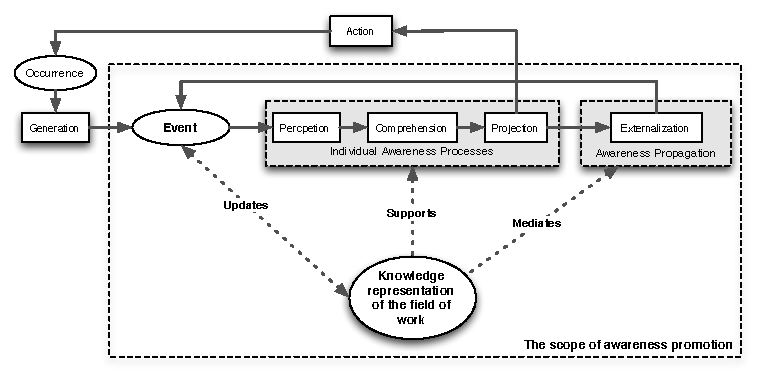
\includegraphics{awareness_promotion_framework.pdf} 
   \caption{Awareness promotion framework}
   \label{fig:awareness_promotion_framework}
\end{figure}

On one hand is how the computer constructs and develops the knowledge representation of the collaborative activities within the event-driven processes. In order to model the development of collaborative activities, the computational representation should support dynamic adaptation so that it always reflects the current state of the changing environment. As human actors use a subset of the awareness information to develop their individual awareness, the system processes the awareness information that is available in the whole collaborative activity. The awareness information can be generated by sensing the occurrences in real world, or it can be the results of human actors' externalization of their individual awareness. All of the awareness information will be processed by the computer system to update its knowledge representation of the collaborative activity.

On the other hand, the knowledge representation is used by the computer system to promote the awareness processes. In general, the role of the computer system is to strike a balance between the system's reasoning capabilities and providing visual and interactive support. With the computational knowledge about the collaborative activities, the system can offload some of the reasoning effort from the human actors. Meanwhile, the systematic knowledge can also be visualized to help the human actors to develop their individual awareness or externalize it for awareness transactions. 

Following of this section discusses the major design choices of these two components, but leave their details to next two chapters respectively.
% subsection the_awareness_promotion_framework (end)

\subsection{Computational knowledge representation} % (fold)
\label{sub:computational_knowledge_representation}
The nature of awareness phenomena in distributed, complex collaboration as we conceptualized in Section \ref{cha:the_conceptual_framework}, and the goal of promoting awareness impose several requirements for the knowledge representation of the collaborative activity:

\begin{enumerate}
   \item The representation should encode enough knowledge about collaborative activities, including all the three constructs in our conceptual model, i.e. the basic elements and relations in collaborative activities, the local scopes of work for actors, and the various dependency relationships among actions. 
   \item The knowledge representation should be dynamically updated. Since the awareness needs of users change quickly with the development of collaborative activities, it is essential that the knowledge representation should be kept updating so that it always reflects the current state of the changing activities.
   \item The knowledge representation needs to be formalized and can be computationally modeled so as to support reasoning.
\end{enumerate}

Existing awareness systems have provided several approaches to representing the collaborative work. The AREA system \cite{fuchs1999a} models the collaborative work as semantic networks including relations among objects, where objects can be human actors artifacts, or aggregations such as groups of people. The representation is primarily used for the users to specify which objects and associated events they are interested in and when they want to be informed. The Atmosphere model \cite{Rittenbruch2002} describes the collaborative work as a hierarchically structured workspace that consists of a set of \emph{spheres} and \emph{sub-spheres}. Users classify their actions on artifacts by mapping them into different spheres. The MoMA model \cite{simone2002a} applies a reaction-diffusion metaphor to model the collaborative work as a set of entities embedded in an interaction space, which behave by using diffusion and reaction capabilities. This metaphor is based on the idea that whenever two or more entities have contact, their states are modified in some way. Their states are then propagated to others through fields in the space.  

Although these representations have shown their capabilities to support specific aspects of awareness in their respective application domains, none of them can meet all the three requirements for knowledge representation to enable awareness promotion. The AREA model provides a good representation of the actions and the dependencies using the semantic networks, but the local scopes of actors are not captured. The model is static (as it is pre-determined by the designers), and informal (as it is primarily used as a descriptive framework). The Atmosphere model organizes the field of work around the artifacts without explicit representation of actions. It supports the specification of each user's local scope using private `spheres', but no dependency relationships between actions are supported. It supports the modification to the representation by human users, but the system cannot automatically adapt the representation to the changing environment. The MoMA model can support all the three constructs of the field of work as the definition of entities and spaces are generic, and provide some reasoning capabilities. However, it does not support the dynamical adaptation of the model.

In this study we draw knowledge representation and reasoning techniques from existing studies in artificial intelligence to develop a computational model of the collaborative activities that can satisfy all the three requirements. An important feature of our model is the capability to model intentions, beliefs, knowledge, and other attributes of actors' mental states \cite{grosz1996collaborative}. As human actors' awareness processes are directed by their mental models, we believe that understanding and representing human actors' mental states allow the computer to infer each actor's local scope, and derive awareness needs from it. 
% subsection computational_knowledge_representation (end)

\subsection{Event driven awareness processes} % (fold)
\label{sub:event_driven_awareness_processes}
In our approach, we adopt the general event-driven interaction paradigm \cite{Etzion2010} to model the awareness processes. In the event-driven mode of interaction, actors (both human and computer) communicate by generating and receiving events. Each actor receives events from environment and other actors, reacts to them, and generates new events to other actors. We believe that the event-driven paradigm is suitable for modeling awareness processes in our study for two major reasons:

\begin{enumerate}
   \item The event-driven paradigm opens up the opportunities for active promotion by the computational system. Instead of asking the human actors to monitor the environment and pull awareness information from it, events are pushed to them. The information push allows the system to take control and present the awareness information to the actors before they subscribe to them.
   \item As awareness information is explicitly represented as first-class objects in event-driven approaches, this allows for representing any aspects of the collaborative activities, not only the external aspects, but also the internal aspects reflecting intentions and beliefs of the actors.
\end{enumerate}

\subsubsection{The concept of event} % (fold)
\label{ssub:the_concept_of_events}
Before going further we should clarify what we mean by an event. The concept of `event' has been used in the literature from different perspectives:

\begin{enumerate}
   \item The first meaning refers to an actual occurrence (the something that has happened) in the real world. Set out by Quine \cite{quine1985events}, events in this meaning are first-class entities that can be localized in space and time, broken into sub-parts, and arranged in a taxonomic hierarchy. Research using this concept of events primarily focuses on studying the internal structures of the events. For example, in \cite{Yuan2001}, complex geographical phenomena, such as wildfire or precipitation, have been modeled in a hierarchy of events, processes, and states. In \cite{Andrienko2011}, the event-based approach has been adopted to model all the types of occurrences in movement analysis. The focus here is to derive the different event types that may occur and identify the relationships between them.
   \item The second meaning takes us into the realm of computerized event processing, where the word `event' is used to mean a programming entity that represents this occurrence \cite{Spiteri2000}. Each event in this notion is a message that describes a real world occurrence by its source, location, time, and other measurable properties. A single event occurrence can be represented by many event entities, and a given event entity might capture only some of the facets of a particular event occurrence \cite{Etzion2010}.
   \item In event-based awareness systems, the concept of event has a more specific meaning as representing a specific type of awareness information that might be relevant to the user's work. It is usually an application-specific concept, depending on the set of awareness information that is supported by an awareness system. For instance, the AREA system \cite{fuchs1999a} describes events as actions performed on an artifact and the event classes are derived from the artifact class hierarchy and possible operations on them. The ENI system \cite{Gross2004} describes events from the sensors associated with actors, shared artifacts, or any other objects that generate events related to them. 
\end{enumerate}

In this study, we use three different words to avoid the confusion when defining events:
\begin{enumerate}
   \item We use the word \emph{`occurrence'} to denote the real world happenings. It can be in the environment, e.g. the occurrence of a traffic accident at a location; or associated with an object, e.g. a vehicle arrives at the accident spot; or associated with human actions, e.g. the successful performance of first aid on a victim. 
   \item The word \emph{`awareness'} is used to refer to the human consciousness about the occurrences, events, and their relevance to ongoing or future human activities. It emphasizes that awareness is inherently a cognitive, interpretive, and predicative concept that reflects a state of mind.
   \item We use the word \emph{`event'} to denote a computerized entity that describes a piece of awareness information that is relevant to an actor's work. On one hand, it can be the description of a real world \emph{occurrence} by its measurable properties, e.g. the information about a traffic accident with time, location, number of victims etc. On the other hand, it can also be the externalization of an actor's \emph{awareness} knowledge, e.g. an actor's belief that the accident will block the traffic and cause a delay on delivery of medical team.
\end{enumerate}
% subsubsection the_concept_of_event (end)

\subsubsection{Awareness processes} % (fold)
\label{ssub:awareness_processes}
Along with the distinction between the concepts of \emph{`occurrence'}, \emph{`awareness'}, and \emph{`event'} is the notion of dynamic transformations between them (Figure \ref{fig:occurrence_event_awareness}). The transformations are tied to different processes in awareness development. 

\begin{figure}[htbp] %  figure placement: here, top, bottom, or page
   \centering
   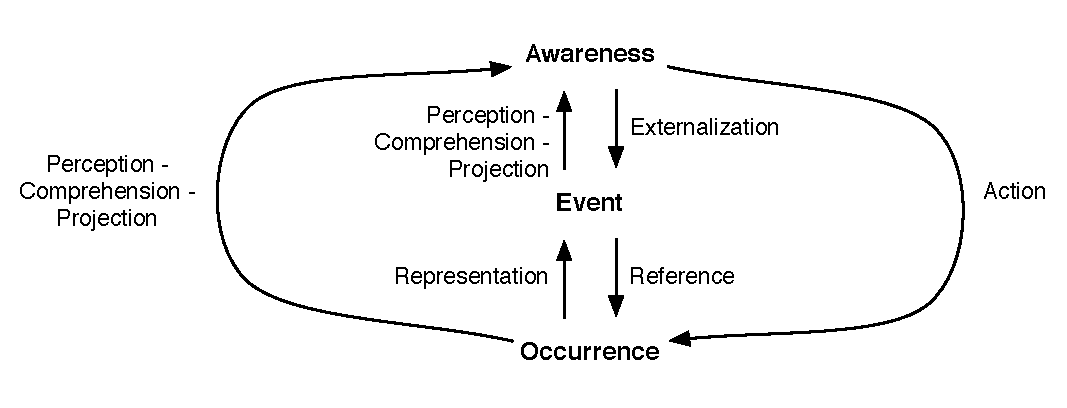
\includegraphics[width=4.5in]{occurrence_event_awareness.pdf} 
   \caption{Transformations between occurrence, event, and awareness}
   \label{fig:occurrence_event_awareness}
\end{figure}

The direct transformation between \emph{occurrence} and \emph{awareness} corresponds to the individual awareness development cycle that has been described in Section \ref{sec:development_of_awareness}. A real world \emph{occurrence} is transformed into \emph{awareness} through an actor's individual awareness processes, i.e. \emph{perception}, \emph{comprehension}, and \emph{projection}. Then, the achieved \emph{awareness} guides the actor's \emph{action} that may generate further \emph{occurrences} in the real world. 

The thing becomes more interesting when the computer support is involved and the transformations are driven by \emph{events}. On one hand is a real world \emph{occurrence} can be captured and represented as an \emph{event} by the computer system, and presented to a human actor. Instead of perceiving the \emph{occurrence} directly, the actor perceives the corresponding \emph{event} in the computer interface, and develops the \emph{awareness} upon it through the actor's individual awareness processes, i.e. \emph{perception}, \emph{comprehension}, and \emph{projection}. On the other hand is some aspect of the actor's \emph{awareness} can be externalized as a new \emph{event}, which refers to some current \emph{occurrence} or predicts future \emph{occurrence} in the real world.

The event-driven transformations can also be used to describe the different types of awareness transactions across multiple actors. The process of \emph{mutual monitoring} can then be described in the following steps: (1) an actor's \emph{awareness} guides his/her \emph{action} that generates a new \emph{occurrence} in the real world; (2) this new \emph{occurrence} is then captured and represented as an \emph{event} by the computer, and presented to another actor; (3) the other actor develops the \emph{awareness} upon receiving the new event. Similarly, the process of \emph{externalization} can also be described as follow: (1) an actor's \emph{awareness} is externalized as a new \emph{event}, which refers to some current \emph{occurrence}; (2) this new \emph{event} is then presented to another actor by the computer; (3)the other actor develops the \emph{awareness} upon receiving the new event. 

Figure \ref{fig:example_awareness_traj} shows an example of how these event-driven awareness processes can be combined together to describe a developmental trajectory of awareness that involves three actors in a group. The awareness is propagated from $Actor1$ to $Actor2$ through the process of \emph{externalization}, and is then propagated from $Actor2$ to $Actor3$ through the process of \emph{mutual monitoring}.

\begin{figure}[htbp] %  figure placement: here, top, bottom, or page
   \centering
   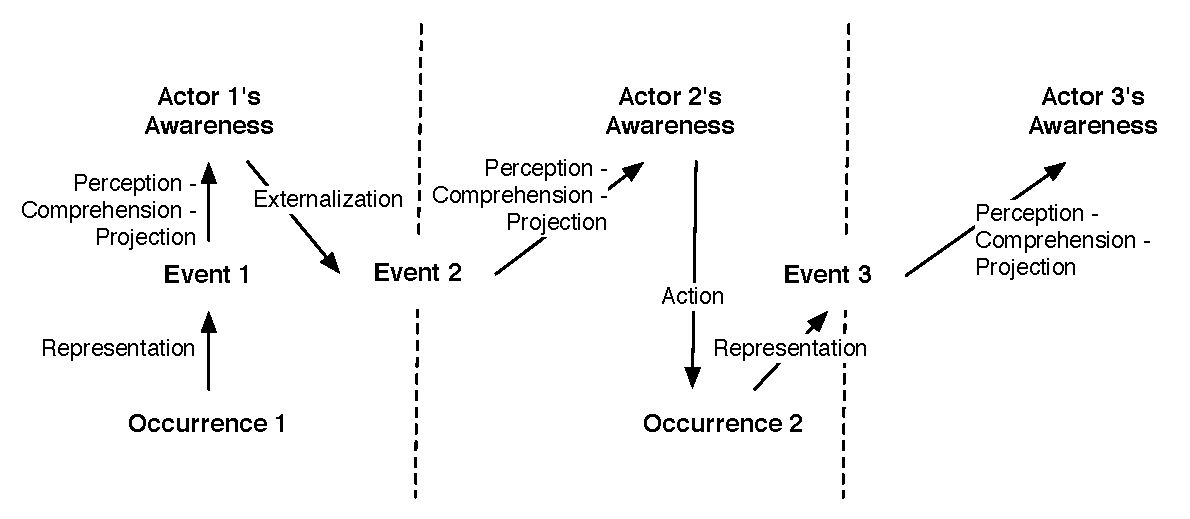
\includegraphics[width=4.5in]{example_awareness_traj.pdf} 
   \caption{An example of event-driven developmental trajectory}
   \label{fig:example_awareness_traj}
\end{figure}
% subsubsection awareness_processes (end)
% subsection event_driven_awareness_processes (end)
% section awareness_promotion_approach (end)

\section{Discussion} % (fold)
\label{sec:discussion}
In this chapter, we first identify the major challenges for human actors to achieve and develop awareness in distributed, complex collaborative activities, which highlight the design aspects in which computer systems can provide support to augment and complement human capability at both the individual and team levels. 

The analysis of the design aspects provides us the basis to review existing awareness support systems. The purpose of the review, however, is not to provide an exhaustive evaluation on existing studies. Instead, we use the review to understand how the design aspects have been addressed or partially addressed in existing awareness support systems, and identify the major limitations:

\begin{enumerate}
   \item Existing systems to support awareness processes are usually designed to support collaborative activities at relatively small and medium scales, it becomes a much more difficult task to support awareness in complex, distributed activities as we are interested in this study. On one hand, space-based models rely on the users to monitor the shared spaces and perceive the awareness information. This provides more flexibility to handle increased level of dynamics, but at the same time it becomes  problematic when the collaborative is scaled up with higher level of complexity and actions of users are highly distributed. On the other hand, event-based systems are more efficient to handle higher-level of complexity as the users can decide on what aspects of awareness information that should be presented, and they do not need to switch their attentions to other's actions until the event notification happens. However, event-based systems become less effective in high level of dynamics as the user's awareness needs are often in the flux of changes.
   \item The support for various awareness processes at both the individual and collaborative levels is limited. At the individual level, existing awareness systems have focused on supporting perception, the higher level of awareness processes are relatively less supported. At the team level, existing awareness systems have focused on either supporting the explicit communication among human collaborators, or different approaches to providing `shared spaces' so that the actions of each other become visible to each other. However, less discussion has been given to support explicit representation of transactive knowledge, or the externalization process.
\end{enumerate}

Motivated by these limitations, we argue that the computer system needs to play a more active role to promote awareness among collaborators, and provide an overview the awareness promotion approach. We believe the characteristics of awareness promotion approach provide the potential to address limitations of existing awareness systems to handle the scaled up complexity and dynamics, and to provide integrated awareness support. First, the awareness promotion approach utilizes the computational knowledge representation to model the collaborative activities and offloads some of the representation and reasoning efforts from the human to the computer. Hence, it can  handle more complex collaborative configurations than existing awareness models. Meanwhile, the knowledge representation is dynamically updated to reflect the current state of the collaborative work, which allows it to handle increased level of dynamics. Last, as the computer's knowledge representation is at the team level and is equipped with the computational reasoning capabilities, it allows the computer to provide support on both the higher level of individual awareness processes and awareness transactions.

The next two chapters provide details of this awareness promotion framework. Chapter \ref{cha:knowledge_reprsentation_and_updating} describes the knowledge components, i.e. the computational representation of the collaborative activities and the specification of events, and the mechanisms for updating the knowledge representation with events. Chapter \ref{cha:promoting_event_driven_awareness} describes the different promotion strategies making use of the knowledge representation.
% section discussion (end)
% chapter awareness_promotion (end)



 

